%%%%%%%%%%%%%%%%%%%%%%%%%%%%%%%%%%%%%%%%%
% University Assignment Title Page 
% LaTeX Template
% Version 1.0 (27/12/12)
%
% This template has been downloaded from:
% http://www.LaTeXTemplates.com
%
% Original author:
% WikiBooks (http://en.wikibooks.org/wiki/LaTeX/Title_Creation)
%
% License:
% CC BY-NC-SA 3.0 (http://creativecommons.org/licenses/by-nc-sa/3.0/)
% 
% Instructions for using this template:
% This title page is capable of being compiled as is. This is not useful for 
% including it in another document. To do this, you have two options: 
%
% 1) Copy/paste everything between \begin{document} and \end{document} 
% starting at \begin{titlepage} and paste this into another LaTeX file where you 
% want your title page.
% OR
% 2) Remove everything outside the \begin{titlepage} and \end{titlepage} and 
% move this file to the same directory as the LaTeX file you wish to add it to. 
% Then add \input{./title_page_1.tex} to your LaTeX file where you want your
% title page.
%
%%%%%%%%%%%%%%%%%%%%%%%%%%%%%%%%%%%%%%%%%
%\title{Title page with logo}
%----------------------------------------------------------------------------------------
%	PACKAGES AND OTHER DOCUMENT CONFIGURATIONS
%----------------------------------------------------------------------------------------

\documentclass[12pt]{article}
\usepackage[english]{babel}
\usepackage[utf8x]{inputenc}
\usepackage{amsmath}
\usepackage[colorinlistoftodos]{todonotes}
\usepackage{hyperref}
\setlength {\marginparwidth }{2cm}
\usepackage{adjustbox}
\usepackage{multirow}
\usepackage{float}
\usepackage{listings}
\usepackage[font=small]{caption}
\usepackage{graphicx}
\usepackage{caption}
\usepackage{subcaption}
%%

\begin{document}

\begin{titlepage}

\newcommand{\HRule}{\rule{\linewidth}{0.5mm}} % Defines a new command for the horizontal lines, change thickness here

\center % Center everything on the page
 
%----------------------------------------------------------------------------------------
%	HEADING SECTIONS
%----------------------------------------------------------------------------------------

\textsc{\LARGE Università degli studi di Milano-Bicocca}\\[1cm] % Name of your university/college
\textsc{\Large Advanced Machine Learning }\\[0.3cm] % Major heading such as course name
\textsc{\large Final Project}\\[0.1cm] % Minor heading such as course title

%----------------------------------------------------------------------------------------
%	TITLE SECTION
%----------------------------------------------------------------------------------------

\HRule \\[0.4cm]
{ \huge \bfseries Costa Rican Household Poverty}\\[0.4cm] % Title of your document
\HRule \\[1.5cm]
 
%----------------------------------------------------------------------------------------
%	AUTHOR SECTION
%----------------------------------------------------------------------------------------

\large
\emph{Authors:}\\
Alice Romagnoli - 829833 - a.romagnoli7@campus.unimib.it \\   % Your name
Artemisia Sarteschi - 829677 - a.sarteschi@campus.unimib.it \\ % Your name
Andrea Infantino - 816786 - a.infantino@campus.unimib.it   \\[1cm]
% If you don't want a supervisor, uncomment the two lines below and remove the section above
%\Large \emph{Author:}\\
%John \textsc{Smith}\\[3cm] % Your name

%----------------------------------------------------------------------------------------
%	DATE SECTION
%----------------------------------------------------------------------------------------

{\large \today}\\[1cm] % Date, change the \today to a set date if you want to be precise

%----------------------------------------------------------------------------------------
%	LOGO SECTION
%----------------------------------------------------------------------------------------


\includegraphics{logo.png}\\[1cm] % Include a department/university logo - this will require the graphicx package
 
%----------------------------------------------------------------------------------------

\vfill % Fill the rest of the page with whitespace

\end{titlepage}


\begin{abstract}
%The ABSTRACT is not a part of the body of the report itself. Rather, the abstract is a brief summary of the report contents that is often separately circulated so potential readers can decide whether to read the report. The abstract should very concisely summarize the whole report: why it was written, what was discovered or developed, and what is claimed to be the significance of the effort. The abstract does not include figures or tables, and only the most significant numerical values or results should be given.


Il progetto è volto alla realizzazione di una rete neurale, appositamente costruita per l'identificazione delle persone in stato di povertà nel Costa Rica. Dopo un estesa analisi preliminare e la creazione della rete vengono sperimentate diverse configurazioni di regolarizzazione per gestire l'overfitting, ottenendo dei risultati abbastanza buoni in termini di accuracy ma non pienamente soddisfacenti.

\end{abstract}

\section{Introduzione}
%\textit{The introduction should provide a clear statement of the problem posed by the project, and why the problem is of interest. It should reflect the scenario, if available. If needed, the introduction also needs to present background information so that the reader can understand the significance of the problem. A brief summary of the hypotheses and the approach your group used to solve the problem should be given, possibly also including a concise introduction to theory or concepts used later to analyze and to discuss the results.}


L'analisi condotta è volta a costruire una rete neurale che possa identificare quali persone, tra quasi 10'000 persone costaricane esaminate, si trovino in uno stato di povertà ed abbiano bisogno di assistenza. Il dataset utilizzato riporta per ogni persona una serie di informazioni personali e familiari.
A un'estesa analisi delle variabili, volta a capire quante di queste fossero effettivamente utili e significative, eventualmente aggregandole, sono seguite due diverse tecniche di preprocessing dei dati (FAMD e OHE) volte ad ottenere rappresentazioni utili a rendere più efficace l'addestramento della rete neurale. 
Scelto il preprocessing migliore, sono quindi state sperimentate diverse tipologie di reti e di regolarizzazioni per attenuare l'overfitting: \textit{L1}, \textit{L2}, \textit{Dropout}, \textit{Early Stopping} ed una tecnica per gestire lo sbilanciamento della classe target chiamata \textit{Class Weight}.
\section{Datasets}
%\textit{In this section the available data sets must be presented. The term dataset refers to any type of information source, for example web services for geolocation fall into this category.}
%\textit{In addition, all necessary data manipulation processes, such as cleaning and enrichment with external sources, must be presented and discussed.}




Il dataset scelto per il nostro progetto \textit{Costa Rican Household Poverty Level Prediction} è reperibile su Kaggle \cite{kaggleCostaRican} e contiene tutte le informazioni relative ad un campione di famiglie che vivono in Costa Rica. Il numero di record che compongono il dataset è 9557 e gli attributi sono 143: ogni record rappresenta una singola persona appartenente ad una determinata famiglia.
La variabile target, che si vuole predire, rappresenta il livello di ricchezza/povertà della famiglia di appartenenza dei vari individui, mentre le altre colonne contengono informazioni riguardanti l'individuo o la sua famiglia.
Sul dataset è stato eseguito un importante preprocessing al fine di analizzare e gestire i missing values e di capire il significato, la distribuzione e l'eventuale utilità dei numerosi attributi presenti, spesso denominati in spagnolo. 

\subsection{Metodi Implementati per l'Analisi delle Variabili}
%[inserire le varie immagini]\\
Durante l'analisi sono stati implementati vari metodi per analizzare e visualizzare la distribuzione delle singole variabili. 
Il metodo \texttt{num\_variable()} viene applicato per l'analisi delle variabili con valori numerici, anche ordinali. Nel caso si rivelasse necessario, il metodo procede a cambiare il nome della variabile ed esegue un'analisi: conta le occorrenze per ogni classe o esegue una descrizione statistica. Infine, riporta il numero di missing values riscontrati. 
Il metodo \texttt{plot\_num\_variable()} viene utilizzato per visualizzare graficamente la distribuzione di una variabile numerica o ordinale. In particolare, i parametri \texttt{many\_values} e \texttt{nonzero} permettono di adattare il grafico alle esigenze della singola variabile.
%\texttt{many\_values == True} viene utilizzata quando si hanno molti valori sull'asse x, mentre \texttt{nonzero == True} quando nessun record assume il valore 0. 
Il metodo \texttt{single\_column()} è stato implementato per passare da una rappresentazione one hot encode di più colonne a una singola colonna contenente come valori i nomi delle singole colonne. 
Il metodo \texttt{cat\_variable()} viene impiegato nelle variabili categoriche (binarie o con stringhe come valori). Effettua se necessario due operazioni: rinomina le colonne e raggruppa più colonne in una singola colonna. Riporta poi il numero di missing values e il conteggio delle occorrenze per ogni classe.
Da ultimo, il metodo \texttt{plot\_cat\_variable()} serve per visualizzare la distribuzione di una variabile binaria o con stringhe come valori. I parametri \texttt{binary} e \texttt{central} sono adoperati per adattare meglio il grafico alla variabile.
%Il parametro \texttt{binary} serve a distinguere questi due casi e utilizzare il giusto grafico, mentre il parametro \texttt{central} è adoperato per avere una migliore leggibilità del grafico.

\subsection{Le Variabili del Dataset}

La variabile \texttt{idhogar} (rinominata \texttt{id\_family}), che riporta gli identificativi di 2988 famiglie, permette di capire la distribuzione del numero di componenti per ogni famiglia (solitamente 2-4).
\texttt{id\_family} e la variabile \texttt{Id}, rappresentante l'identificativo delle singole persone, verranno in seguito rimosse.

%Questa variabile verrà rimossa in quanto non sarà possibile mantenerla né tramite One Hot Encode (determinerebbe la creazione di quasi 3000 colonne), né trasformandola in una variabile numerica (assumerebbe erroneamente le caratteristiche di una variabile ordinale).

%Viene rimossa anche \texttt{Id}, rappresentante l'identificativo delle singole persone.

\subsubsection{Variabili Numeriche}

La variabile \texttt{v2a1} (\texttt{monthly\_rent\_payment}) rappresenta l' ammontare dell'af-fitto mensile di ogni famiglia.
Data l'elevata presenza di missing values (circa 7000) e  un confronto con un'altra variabile \texttt{type\_of\_contract} per cercare di ricavare il maggior numero possibile di valori mancanti, questa variabile è stata rimossa dal dataset. Le successive riportano valori nuemrici ma ordinali.
La variabile \texttt{age} riporta l'età di ogni persona nel dataset, concentrate  tra gli 0 e i 60 anni.
La variabile \texttt{escolari} (\texttt{education\_years}) riporta gli anni di istruzione per ogni persona (la cui moda è 6 anni). 
Dal dataset sono state rimosse le variabili \texttt{rez\_esc}, numero di anni scolastici indietro per ogni persona, che contiene un altissimo numero di missing values, e \texttt{meaneduc}, numero medio di anni di istruzione degli adulti della famiglia, informazione ricavabile dalle altre variabili.
Le variabili \texttt{hogar\_nin} (\texttt{num\_child-} \texttt{ren}), \texttt{hogar\_adult} (\texttt{num\_adults}) e  \texttt{hogar\_mayor} (\texttt{num\_enderly}) rappresentano rispettivamente il numero di bambini (età inferiore a 19 anni), adulti e anziani (età superiore a 65 anni) presenti in ogni famiglia. Mediamente, le famiglie sono composte da 1/2 bambini, 2/3 adulti e 0 anziani.
Dalla combinazione di queste variabili è possibile ricavare il numero totale di persone presenti all'interno della famiglia, rendendo superflue le variabili \texttt{r4t3}, \texttt{tamhog}, \texttt{tamviv}, \texttt{hhsize} e \texttt{hogar\_total}. Infine, viene eliminata anche \texttt{dependecy}, che riporta il rapporto tra il numero di bambini o anziani e il numero di adulti per famiglia. 
Le variabili \texttt{rooms} e \texttt{bedrooms} indicano rispettivamente il numero di stanze e camere da letto presenti nelle case di ogni famiglia.
Le informazioni riportate da queste variabili congiunte con il numero di persone in ogni famiglia rendono superflue le variabili: \texttt{overcrowding}, numero di persone per stanza, \texttt{hacdor}, presenza di sovraffollamento riferito al numero di camere da letto e \texttt{hacapo}, presenza di sovraffollamento riferito al numero di stanze.
Le variabili \texttt{r4m3} (\texttt{tot\_females}) e \texttt{r4h3} (\texttt{tot\_males}) riportano rispettivamente il numero di donne e uomini all'interno della famiglia (mediamente due femmine e due maschi).
Vengono quindi rimosse alcune variabili ottenute combinando informazioni riguardanti genere e età dei componenti della famiglia (\texttt{r4h1}, \texttt{r4h2}, \texttt{r4m1}, \texttt{r4m2}, \texttt{r4t1}, \texttt{r4t2}).
La variabile \texttt{hv18q1} (\texttt{num\_tablets}) riporta il numero di tablet per ogni famiglia, riconducibili all'assenza degli stessi e pertanto sotituiti con il valore 0.
La variabile \texttt{qmobilephone} (\texttt{num\_phones}) riporta il numero di telefoni presenti nella famiglia, mediamente 2/3 a famiglia.
Le variabili \texttt{edjefe} e \texttt{edjefa} (unite in \texttt{household\_head\_education}) riportano gli anni di istruzione del capo famiglia. Esse contenevano, oltre a valori numerici, anche i valori \textit{yes} e \textit{no}, sostituiti con i valori numerici 1 e 0.

\subsubsection{Variabili Binarie}

La variabile \texttt{v14a} (\texttt{has\_bathroom}) e  \texttt{refrig} (\texttt{has\_refrigerator}) indicano rispettivamente la presenza o assenza del bagno e del frigorifero all'interno della casa della famiglia.
Le variabili \texttt{v18q} (\texttt{has\_tablet}), \texttt{mobilphone} (\texttt{has \_phone}), \texttt{computer} (\texttt{has\_computer}),  \texttt{television} (\texttt{has\_television}), indicano se la famiglia dell' individuo considerato possiede o meno tablet, computer, televisione e telefono.
La maggior parte delle famiglie non dispongono di questi dispositivi, ad eccezione del telefono.
La variabile \texttt{cielorazo} (\texttt{has\_ceiling}) indica la presenza o assenza del soffitto nella casa.
La variabile \texttt{dis} (\texttt{is\_disabled}) indica se l'individuo considerato è disabile.

\subsubsection{Variabili Categoriche}

Le variabili \texttt{female} e \texttt{male} (unite in \texttt{gender}) rappresentano il genere dell'indi-viduo, la cui quantità nel campione è bilanciata.
Le 7 variabili \texttt{estadocivl} (unite in \texttt{marital\_status}) riportano lo stato civile dell'individuo considerato (in maggioranza single e sposati).
Le 12 variabili \texttt{parentesco} (aggregate in \texttt{relationship}) riportano il grado di parentela che lega ogni individuo al capofamiglia (in maggioranza figli del capofamiglia). Le 9 variabili \texttt{instlevel} (unite in \texttt{education}) rappresentano il tipo di istruzione conseguita da ogni persona.
Le 8 variabili \texttt{pared} (unite in \texttt{outside\_wall}), le 6 \texttt{piso} (unite in \texttt{floor}) e le 4 \texttt{techo} (unite in \texttt{roof}) riguardano il materiale con cui sono fatte rispettivamente le pareti, il pavimento e il tetto dell'abitazione dell'individuo. 
Le 3 variabili \texttt{abastagua} (aggregate in \texttt{water\_provision}), le variabili \texttt{public}, \texttt{planpri}, \texttt{noelec} e \texttt{coopele} (unite in \texttt{electricity\_source}), le 5 variabili \texttt{sanitario} (unite in \texttt{toilet\_system}), le 4 \texttt{energcocinar} (unite in \texttt{energy}) e le 6 \texttt{elimbasu} (unite in \texttt{rubbish\_disposal}) riportano rispettivamente la tipologia di: approvvigionamento dell'acqua, di impianto elettrico, di sistema di servizi igienici, di cucina e di sistema smaltimento dei rifiuti. 
Le 3 variabili \texttt{etecho} (unite in \texttt{roof} \texttt{status}), le 3 \texttt{eviv} (unite in \texttt{floor} \texttt{status}) e le 3 \texttt{epared} (unite in \texttt{walls\_status}), indicano rispettivamente lo stato del tetto, del pavimento e delle pareti dell'abitazione.
Le 5 variabili \texttt{tipoviv} (aggregate in \texttt{type\_of\_contract}) indicano la tipologia di contratto che la famiglia ha stipulato per la casa. La maggioranza sono case di proprietà, seguite da quelle affittate. 
Le 6 variabili \texttt{lugar} (unite in \texttt{region}) e le 2 \texttt{area} rappresentano rispettivamente la regione e l'area in cui risiede l'individuo. 

\subsubsection{Variabile Target}
La variabile \texttt{target} (Figura \ref{fig:distrTarget}) riporta il grado di povertà/ricchezza, e quindi di vulnerabilità, della famiglia dell'individuo. 
Essa può assumere i valori: 1 - povertà estrema, 2 - povertà moderata, 3 - famiglia vulnerabile e 4 - famiglia non vulnerabile.
Il 63\% degli individui appartiene a famiglie non vulnerabili, determinando un dataset un po' sbilanciato.

\begin{figure}[H]
     \centering
     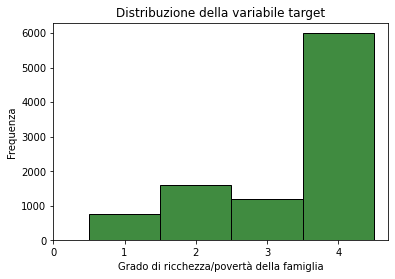
\includegraphics[scale=0.5]{Latex template for Project Report-20220108/immagini/distribuzione target.png}
     \caption{Distribuzione della variabile target}
     \label{fig:distrTarget}
\end{figure}


\section{Approccio Metodologico}

%\textit{This is the central and most important section of the report. Its objective must be to show, with linearity and clarity, the steps that have led to the definition of a decision model. The description of the working hypotheses, confirmed or denied, can be found in this section together with the description of the subsequent refining processes of the models. Comparisons between different models (e.g. heuristics vs. optimal models) in terms of quality of solutions, their explainability and execution times are welcome. }

%\textit{Do not attempt to describe all the code in the system, and do not include large pieces of code in this section, use pseudo-code where necessary. Complete source code should be provided separately (in Appendixes, as separated material or as a link to an on-line repo). Instead pick out and describe just the pieces of code which, for example:
%\begin{itemize}
%\item are especially critical to the operation of the system;
%\item you feel might be of particular interest to the reader for some reason;
%\item  illustrate a non-standard or innovative way of implementing an %algorithm, data
%structure, etc..
%\end{itemize}}

%\textit{You should also mention any unforeseen problems you encountered when implementing the system and how and to what extent you overcame them. Common problems are: difficulties involving existing software.} \\
 



Il dataset, ottenuto al termine della fase di analisi, risulta composto da 39 features rispetto alle 143 di partenza.
Viene quindi effettuata una fase di preprocessing allo scopo di ottenere una rappresentazione dei dati processabile efficacemente dalla rete neurale. Vengono tentati due approcci differenti: \textit{Factor Analysis of Mixed Data (FAMD)} \cite{famd} e  \textit{One Hot Encode (OHE)}. 
FAMD è un principal component method dedicato all'analisi di dataset contenenti variabili sia qualitative che quantitative, permettendo di analizzarne la similarità tra gli individui utilizzando variabili di diverso tipo.
Utilizzando i metodi implementati dalla libreria \texttt{prince} viene trasformato l'intero dataset (ad eccezione della variabile target), ottenendo il \textit{dataset FAMD}, composto da 38 features numeriche.
La libreria \texttt{OneHotEncoder} di \texttt{sklearn.preprocessing} ha invece permesso di codificare le features categoriche (non accettate dalle reti neurali) in binarie, ottenendo il \textit{dataset OHE}, composto da 113 colonne.
Per entrambi i dataset, viene eseguita una prima divisione (80-20) in training e test set e una seconda divisione del training in train e validation set (80-20). 
Dopodiché, le variabili target di ogni set sono state scalate nel range 0-3 e codificate con OHE e per il dataset OHE è stato utilizzato \texttt{StandardScaler()} per scalare i dati di train, validation e test, rendendoli comparabili fra loro.


\subsection{Reti neurali senza regolarizzazione}
Vengono eseguite sperimentazioni con i due dataset, per capire quale predica in modo migliore la classe target.
Per ottenere un'inizializzazione dei pesi non randomica è stato fissato un ramdom seed, \texttt{initializer = tf.keras. initializers.GlorotUniform(seed=1234)}, poi utilizzato in ogni modello. 


\subsubsection{Rete OHE}
Il metodo \texttt{NeuralNetwork()} viene definito per creare la rete neurale per il dataset OHE, in seguito citata come ``rete base". 
Si tratta di una rete (vedi Figura \ref{fig:neuralNetwork}) composta da 5 fully connected layer con un numero di neuroni decrescente (128, 64, 32, 16, 4), adatto a un numero alto di feature (113), e con funzione di attivazione \texttt{relu}. Questa specifica struttura della rete è stata scelta in seguito a numerosi tentativi in cui è stato modificato il numero di layer e il numero di neuroni.
Sono stati scelti \texttt{softmax} come funzione di attivazione dell'ultimo layer e \texttt{categorical\_crossentropy} come loss, in quanto opzioni più adatte per eseguire una classificazione su 4 classi. 
L'optimizer \texttt{adam}, invece, è stato scelto perché meglio performante di altri ottimizzatori testati e ha riportato i risultati migliori con il \textit{learning rate} di default. 
Viene inoltre tenuta traccia della metrica \textit{accuracy} per valutare le prestazioni del modello.
La rete base, come tutte le successive, è stata infine addestrata per 300 epoche, al fine di capirne meglio l'andamento su un numero di iterazioni sufficientemente lungo, e un \texttt{batch\_size} di 128, compromesso tra diverse dimensioni, nessuna particolarmente migliore delle altre.

\subsubsection{Rete FAMD}

Il metodo \texttt{NeuralNetwork\_famd()} viene invece definito per creare la rete neurale per il dataset FAMD. Si tratta di una rete composta da 4 fully connected layer con un numero di neuroni decrescente (64, 32, 16, 4), adatto a un numero di feature (38) non molto alto, ottenendo un modello con un numero decisamente minore di parametri. 
Per quanto riguarda tutti gli altri iperparametri sono stati mantenuti gli stessi usati nella rete base.
\begin{figure}[H]
     \centering
     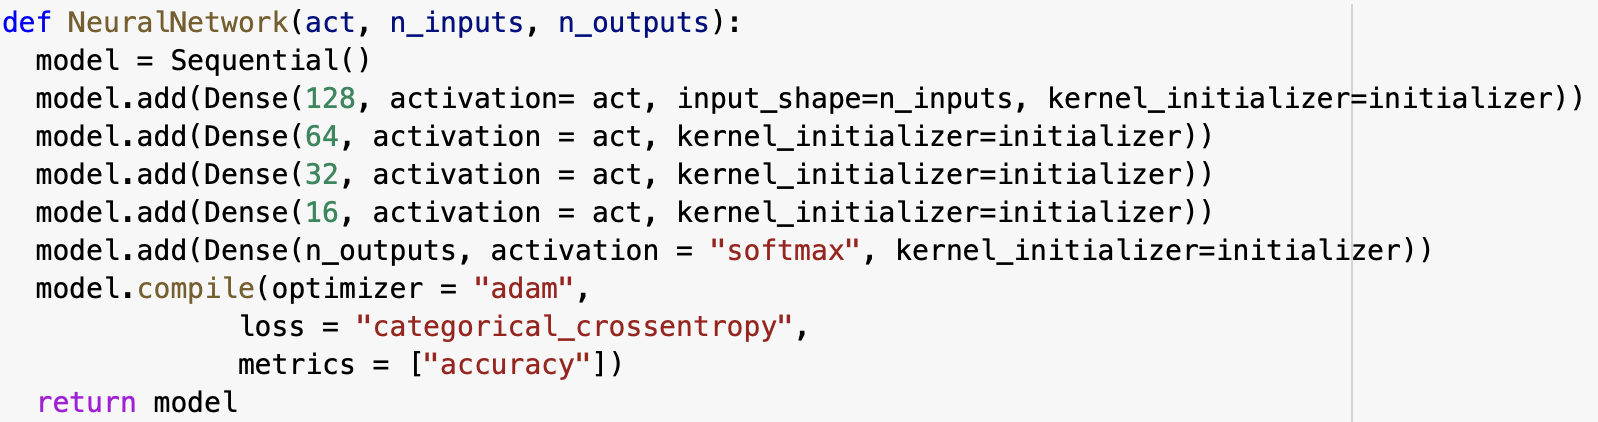
\includegraphics[scale=0.40]{Latex template for Project Report-20220108/immagini/NeuralNetwork.png}
     \caption{Codice metodo Neural Network}
     \label{fig:neuralNetwork}
\end{figure}
Dalle sperimentazioni, il dataset OHE risulta essere quello che
consente di ottenere i risultati migliori (vedi Figura \ref{fig:primiModelli}); motivo per cui verrà impiegato per tutti i successivi test. 
Per migliorare la rete base e contrastare il fenomeno dell'overfitting sono state utilizzate varie tecniche di regolarizzazione (\textit{Dropout}, \textit{L1}, \textit{L2} e \textit{Early Stopping}), mentre per sopperire allo sbilanciamento dei dati è stato usato \textit{Class Weighting}.




%(vedi Figura \ref{fig:modelFit})

% \begin{figure}[H]
%      \centering
%      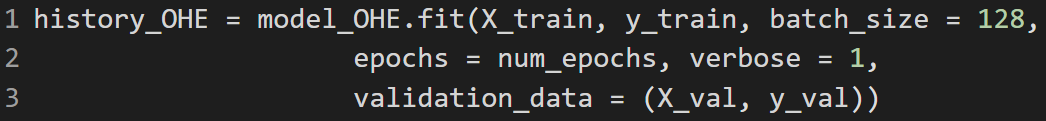
\includegraphics[scale=0.45]{Latex template for Project Report-20220108/immagini/ModelFit.png}
%      \caption{Codice metodo addestramento rete base}
%      \label{fig:modelFit}
% \end{figure}




\subsubsection{Dropout}
La prima tecnica considerata è \textit{Dropout}, metodo di regolarizzazione che permette durante la fase di training di considerare (in alcuni layer) solo una porzione casuale dei neuroni (e rispettive connessioni).
Il metodo che permette di definire la rete neurale base (\texttt{NeuralNetworkDropout()}) aggiungendo dei layer di Dropout dopo il secondo, terzo e quarto layer. Le percentuali di neuroni rimosse, selezionate dopo diversi tentativi, sono le seguenti: 30\% al secondo layer, 20\% al terzo e 10\% al quarto.

\subsubsection{L1 e L2}
Si testano le tecniche \textit{L1}, che usa come funzione di regolarizzazione la somma dei pesi e penalizza maggiormente i pesi più piccoli, e \textit{L2}, che usa la somma dei quadrati dei pesi e penalizza i pesi più grandi.
\texttt{NeuralNetworkL1\_L2()} ridefinisce la rete base aggiungendo la regolarizzazione \textit{L1} o \textit{L2}, determinata attraverso il parametro \texttt{l1} e applicata a ogni layer eccetto l'ultimo. Sia i kernel regularizers che i bias regularizers utilizzano uno stesso valore di regolarizzazione che però cambia tra \textit{L1} e \textit{L2} (rispettivamente 0.001 e 0.01), ed è stato scelto dopo una serie di sperimentazioni.

%I risultati ottenuti da \textit{L1} sono i seguenti: la validation riporta valori di \textit{accuracy} e di \textit{loss} peggiori rispetto a quelli del training set, portando quindi a ipotizzare una situazione di overfitting che abbiamo potuto riscontrare anche nei grafici, visibili nel \href{https://colab.research.google.com/drive/1SPoqJncv_oZZa3kvBMZnVyedcMGaKDti?usp=sharing}{notebook}, in cui la loss del validation set però tende a crescere anziché diminuire. L'accuracy invece si stabilizza su un valore non alto e smette presto di crescere. 

%I risultati ottenuti da \textit{L2} sono i seguenti: la validation riporta valori di \textit{accuracy} e di \textit{loss} peggiori rispetto a quelli del training set, portando quindi a ipotizzare una situazione di overfitting che abbiamo potuto riscontrare anche nei grafici, visibili nel \href{https://colab.research.google.com/drive/1SPoqJncv_oZZa3kvBMZnVyedcMGaKDti?usp=sharing}{notebook}, in cui la loss del validation set però tende a crescere e diminuire leggermente verso le ultime epoche. L'accuracy invece continua a crescere durante le epoche. 
%In generale i valori raggiunti con il validation set sono sufficienti ma non eccellenti in entrambi i modelli. Entrambe le tipologie di regolarizzazione vengono sperimentate su 300 epoche i cui risultati sono riportati nella tabella \ref{table:l1l2}.

\subsubsection{L2 e Dropout}
È stato poi effettuato un tentativo combinando le tecniche di \textit{L2} e \textit{Dropout}, tramite il metodo \texttt{NeuralNetworkL2\_drop()}, per cercare di ottenere risultati migliori. 
Infatti, dall'osservazione dell'andamento della history (Figura \ref{fig:primiModelli}) viene scelto di continuare le sperimentazioni utilizzando \textit{L2}, anziché \textit{L1}.
Per il \textit{Dropout} sono state scelte percentuali più basse in modo da non incidere troppo con la regolarizzazione sul modello. In particolare nel secondo, terzo e quarto strato viene rimosso il 10\% dei neuroni.

%Da cui possiamo notare essere molto simili a quelli precedentemente ottenuti con \textit{L2}, ma la \textit{loss} sul validation set risulta migliore rispetto a quella ottenuta con solo \textit{Dropout}.

\subsubsection{Early Stopping (ES)}
La quarta tecnica di regolarizzazione utilizzata è \textit{Early Stopping} \textit{(ES)} \cite{machinelearningmasteryEarlyStopping}, che consente di ritornare al miglior modello ottenuto durante la fase di training se esso non coincide con l'ultimo ottenuto.
Risulta quindi necessario definire la variabile \texttt{early\_stopping}, che specifica la variabile da monitorare durante il training, \texttt{validation loss}, e la \texttt{patience} da avere prima di decretare che il modello non stia migliorando. 
Dal momento che la loss ha un andamento molto oscillante (vedi Figura \ref{fig:secondiModelli}), è stata fissata una \texttt{patience} alta (70 epoche). Viene definito un \texttt{ModelCheckpoint} per salvare il miglior modello ottenuto nel training, scelto in base ai valori assunti da \textit{validation accuracy}. 
La tecnica \textit{ES} viene quindi aggiunta ai due migliori modelli ottenuti finora: \textit{L2} e \textit{L2} con \textit{Dropout}, vengono addestrate usando gli stessi parametri della rete base con l'aggiunta di \texttt{callbacks} per \textit{ES}.

%\href{https://colab.research.google.com/drive/1SPoqJncv_oZZa3kvBMZnVyedcMGaKDti?usp=sharing}{notebook}

%L'addestramento viene quindi bloccato alla 96esima epoca, la \textit{loss} calcolata sul validation set stava continuando a crescere. 

%Confrontando con i valori di \textit{accuracy} e \textit{loss} ottenuti (riportati nella tabella \ref{table:l2es}) con i valori ottenuto con il modello \textit{L2} senza \textit{Early Stopping} notiamo che i valori ottenuti con il train set sono leggermente peggiori ma comunque molto buoni, mentre la \textit{loss} ottenuta con il \textit{validation set} è migliorata e l'\textit{accuracy} ottenuta con il \textit{validation set} leggermente peggiorata.
%Nel complesso, non sembrano esserci sostanziali differenze tra i due modelli.


%L'addestramento viene bloccato alla 165esima epoca.

%La particolarità di questo addestramento è che neanche dai risultati ottenuti sul \textit{training set} (visibili nella tabella \ref{table:l2dropes}) notiamo particolari miglioramenti nel corso delle epoche.
%Confrontando con i valori di \textit{accuracy} e \textit{loss} ottenuti con il modello \textit{L2} e \textit{Dropout} senza \textit{Early Stopping} notiamo che i valori ottenuti con il train set sono ora leggermente migliori, mentre la \textit{loss} ottenuta con il \textit{validation set} è molto simile e l'\textit{accuracy} ottenuta con il \textit{validation set} è migliorata.
%Nel complesso, anche in questo caso le differenze sono minime. Confrontando invece con i risultati ottenuti con \textit{L2} e \textit{Early stopping} notiamo che per quanto riguarda la \textit{validation}, l'\textit{accuracy} è migliore con il \textit{Dropout}, mentre la \textit{loss} peggiore. 

\subsubsection{Class Weight (CW)}

Al fine di migliorare i risultati ottenuti e gestire lo sbilanciamento della variabile target, viene fatto un tentativo di \textit{Class Weighting (CW)} \cite{kerasKerasDocumentation}\cite{tensorflowClassificazioneDati}. Il metodo \texttt{compute\_class\_weight} di \textit{Keras}, che permette di assegnare un nuovo peso alle classi del target, in modo da bilanciare le loro occorrenze nel dataset: i pesi più alti vengono assegnati alle classi minoritarie.
\textit{CW} e \textit{ES} vengono quindi applicati ai due modelli \textit{L2} e \textit{L2-Dropout}, addestrandole usando gli stessi parametri
della rete base con l'aggiunta di \texttt{callbacks} e  \texttt{class\_weight}.

%\textit{Early Stopping} porta l'addestramento a interrompersi alla 72esima epoca.

%\href{https://colab.research.google.com/drive/1SPoqJncv_oZZa3kvBMZnVyedcMGaKDti?usp=sharing}{notebook}) possiamo notare una crescita della \textit{validation accuracy} e un'iniziale crescita, seguita da una decrescita della \textit{validation loss} (motivo per cui l'addestramento si interrompe dopo così poche epoche). 

%Confrontando con i valori di \textit{accuracy} e \textit{loss} ottenuti (riportati nella tabella \ref{table:l2dropes}) con il modello \textit{L2 Early Stopping} senza \textit{Class Weight}, notiamo che sul training set ora otteniamo valori migliori, mentre sul validation set la \textit{loss} è peggiorata mentre l'\textit{accuracy} e migliorata. 
%Come nei casi precedenti, i risultati dei due modelli confrontati non distano poi molto fra loro.

%\textit{Early Stopping} porta l'addestramento a interrompersi alla 74esima epoca.

%Entrambe \textit{loss} e \textit{accuracy} risultano essere oscillanti, come si può riportare dai grafici riportati nel e dai grafici (riportati nel nel \href{https://colab.research.google.com/drive/1SPoqJncv_oZZa3kvBMZnVyedcMGaKDti?usp=sharing}{notebook}), ma si può notare come la \textit{validation loss} in un primo momento cresce, per poi decrescere. Non sono comunque più stati raggiunti gli iniziali risultati, motivo per cui dopo 70 epoche di non miglioramento, l'addestramento è stato interrotto.

%Confrontando con i valori di \textit{accuracy} e \textit{loss} ottenuti, riportati nella tabella \ref{table:l2escw} con il modello con \textit{L2, Dropout e Early Stopping} ma senza \textit{Class Weight} notiamo che la \textit{training loss} è leggermente peggiorata, mentre la \textit{training accuracy} leggermente migliorata. 
%Stessa situazione riscontriamo anche per \textit{accuracy} e \textit{loss} del \textit{validation set}. 
%Le differenze risultano però essere minime.
%Confrontando invece con i risultati ottenuti con il modello con \textit{L2} e \textit{Early Stopping}, notiamo che per quanto riguarda il training, ora otteniamo risultati migliori, mentre per la \textit{validation} solo l'\textit{accuracy} è di poco migliore.
\section{Risultati e Valutazione}
\label{cap4}
%\textit{The Results section is dedicated to presenting the actual results (i.e. measured and calculated quantities), not to discussing their meaning or interpretation. The results should be summarized using appropriate Tables and Figures (graphs or schematics). Every Figure and Table should have a legend that describes concisely what is contained or shown. Figure legends go below the figure, table legends above the table. Throughout the report, but especially in this section, pay attention to reporting numbers with an appropriate number of significant figures. }

In Figura \ref{fig:primiModelli} e Figura \ref{fig:secondiModelli} vengono riportati i risultati ottenuti sul train e validation set per \textit{loss} e \textit{accuracy} con i modelli precedentemente descritti.
Si può notare come, nonostante vari tentativi con diverse tecniche di regolarizzazione, nessuna rete abbia condotto a risultati soddisfacenti sul validation set.
Il principale problema riscontrato è la tendenza della \textit{validation loss} a una leggera crescita (ciò è osservarvabile in quasi tutti i modelli, nonostante le tecniche di regolarizzazione).
\begin{figure}[h!]
     \centering
     \begin{subfigure}[b]{0.32\textwidth}
         \centering
         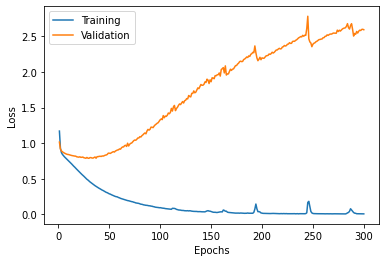
\includegraphics[width=\textwidth]{Latex template for Project Report-20220108/immagini/FAMDLoss.PNG}
         \caption{FAMD Loss}
         \label{fig:FAMDLoss}
     \end{subfigure}
     \hfill
     \begin{subfigure}[b]{0.32\textwidth}
         \centering
         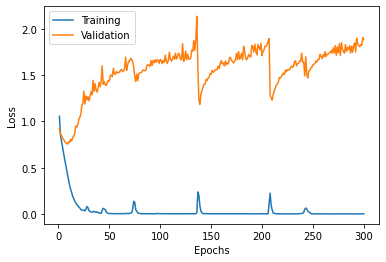
\includegraphics[width=\textwidth]{Latex template for Project Report-20220108/immagini/OHELoss.png}
         \caption{OHE Loss}
         \label{fig:OHELoss}
     \end{subfigure}
     \hfill
     \begin{subfigure}[b]{0.32\textwidth}
         \centering
         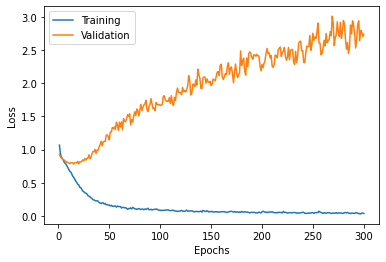
\includegraphics[width=\textwidth]{Latex template for Project Report-20220108/immagini/DropoutLoss.png}
         \caption{Dropout Loss}
         \label{fig:DropLoss}
     \end{subfigure}
     
     \begin{subfigure}[b]{0.32\textwidth}
         \centering
         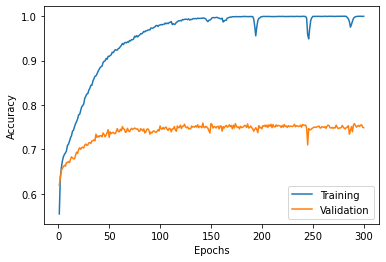
\includegraphics[width=\textwidth]{Latex template for Project Report-20220108/immagini/FAMDAccuracy.png}
         \caption{FAMD Accuracy}
         \label{fig:FAMDAcc}
     \end{subfigure}
     \hfill
     \begin{subfigure}[b]{0.32\textwidth}
         \centering
         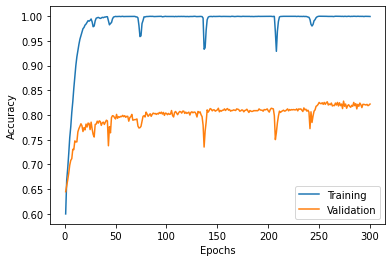
\includegraphics[width=\textwidth]{Latex template for Project Report-20220108/immagini/OHEAccuracy.png}
         \caption{OHE Accuracy}
         \label{fig:OHEAcc}
     \end{subfigure}
     \hfill
     \begin{subfigure}[b]{0.32\textwidth}
         \centering
         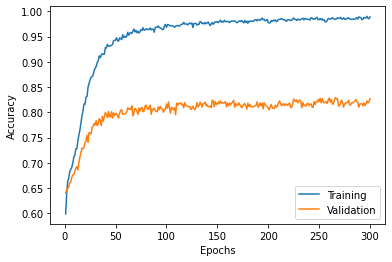
\includegraphics[width=\textwidth]{Latex template for Project Report-20220108/immagini/DropoutAccuracy.png}
         \caption{Dropout Accuracy}
         \label{fig:DropAcc}
     \end{subfigure}
     
     \begin{subfigure}[b]{0.32\textwidth}
         \centering
         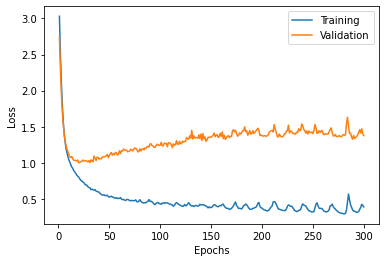
\includegraphics[width=\textwidth]{Latex template for Project Report-20220108/immagini/L1Loss.png}
         \caption{L1 Loss}
         \label{fig:L1Loss}
     \end{subfigure}
     \hfill
     \begin{subfigure}[b]{0.32\textwidth}
         \centering
         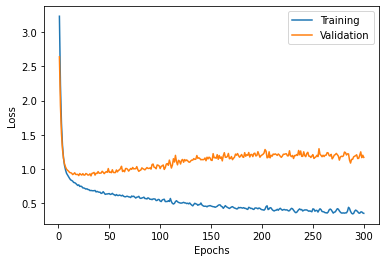
\includegraphics[width=\textwidth]{Latex template for Project Report-20220108/immagini/L2Loss.png}
         \caption{L2 Loss}
         \label{fig:L2Loss}
     \end{subfigure}
     \hfill
     \begin{subfigure}[b]{0.32\textwidth}
         \centering
         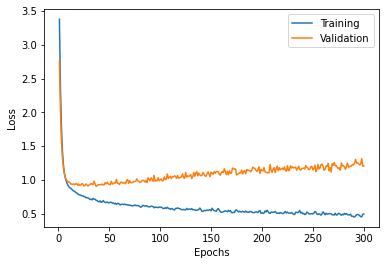
\includegraphics[width=\textwidth]{Latex template for Project Report-20220108/immagini/L2DropoutLoss.png}
         \caption{L2-Drop Loss}
         \label{fig:L2DropLoss}
     \end{subfigure}
     
     \begin{subfigure}[b]{0.32\textwidth}
         \centering
         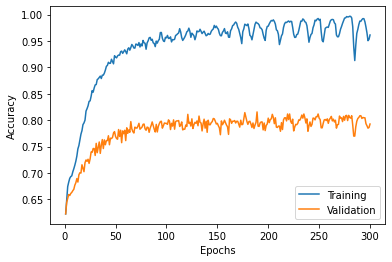
\includegraphics[width=\textwidth]{Latex template for Project Report-20220108/immagini/L1Accuracy.png}
         \caption{L1 Accuracy}
         \label{fig:L1Acc}
     \end{subfigure}
     \hfill
     \begin{subfigure}[b]{0.32\textwidth}
         \centering
         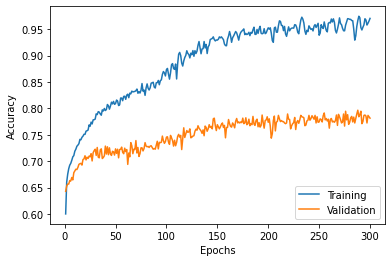
\includegraphics[width=\textwidth]{Latex template for Project Report-20220108/immagini/L2Accuracy.png}
         \caption{L2 Accuracy}
         \label{fig:L2Acc}
     \end{subfigure}
     \hfill
     \begin{subfigure}[b]{0.32\textwidth}
         \centering
         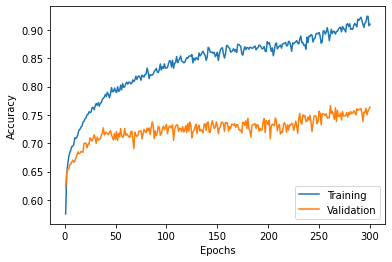
\includegraphics[width=\textwidth]{Latex template for Project Report-20220108/immagini/L2DropoutAccuracy.png}
         \caption{L2-Drop Accuracy}
         \label{fig:L2DropAcc}
     \end{subfigure}

     \caption{Loss e accuracy dei modelli ottenuti con e senza regolarizzazione}
     \label{fig:primiModelli}
\end{figure}
D'altro canto si può invece notare come l'andamento della \textit{validation accuracy} tenda correttamente a crescere (anche se in molti casi non in maniera decisa). Buoni risultati sono invece stati ottenuti sul training set sia per \textit{loss} che per \textit{accuracy}. Al fine di rendere più chiaro il risultato ottenuto all'ultima epoca da ogni modello, sono stati riportati nella Tabella \ref{tab:xxx} i valori di \textit{loss} e \textit{accuracy} per train e validation set.

\begin{figure}[h!]
     \centering
    \begin{subfigure}[b]{0.32\textwidth}
         \centering
         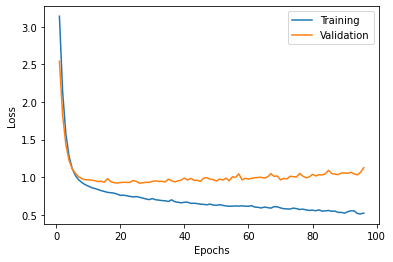
\includegraphics[width=\textwidth]{Latex template for Project Report-20220108/immagini/L2EarlyLoss.png}
         \caption{L2-ES Loss}
         \label{fig:L2ESLoss}
     \end{subfigure}
     \hfill
     \begin{subfigure}[b]{0.32\textwidth}
         \centering
         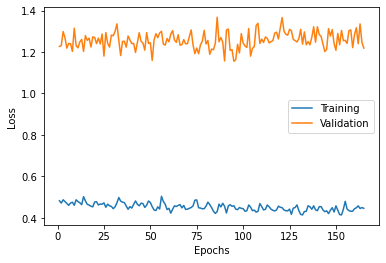
\includegraphics[width=\textwidth]{Latex template for Project Report-20220108/immagini/L2DropEarlyLoss.png}
         \caption{L2-Dr-ES Loss}
         \label{fig:L2DropESLoss}
     \end{subfigure}
     \hfill
     \begin{subfigure}[b]{0.32\textwidth}
         \centering
         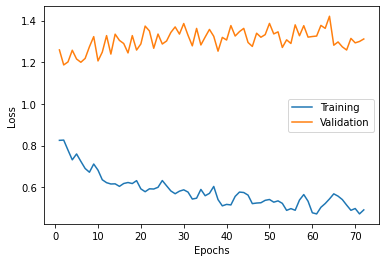
\includegraphics[width=\textwidth]{Latex template for Project Report-20220108/immagini/L2EarlyCWLoss.png}
         \caption{L2-ES-CW Loss}
         \label{fig:L2ESCWLoss}
     \end{subfigure}
     
      \begin{subfigure}[b]{0.32\textwidth}
         \centering
         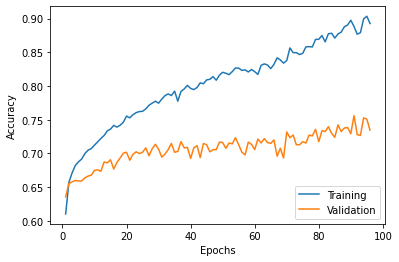
\includegraphics[width=\textwidth]{Latex template for Project Report-20220108/immagini/L2EarlyAccuracy.png}
         \caption{L2-ES Accuracy}
         \label{fig:L2ESAcc}
     \end{subfigure}
     \hfill
     \begin{subfigure}[b]{0.32\textwidth}
         \centering
         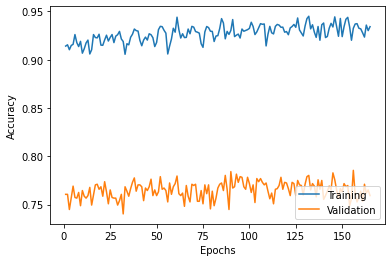
\includegraphics[width=\textwidth]{Latex template for Project Report-20220108/immagini/L2DropEarlyAccuracy.png}
         \caption{L2-Dr-ES Accuracy}
         \label{fig:L2DropESAcc}
     \end{subfigure}
     \hfill
     \begin{subfigure}[b]{0.32\textwidth}
         \centering
         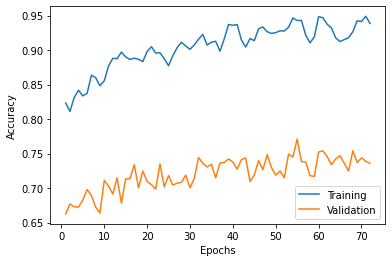
\includegraphics[width=\textwidth]{Latex template for Project Report-20220108/immagini/L2EarlyCWAccuracy.png}
         \caption{L2-ES-CW Acc}
         \label{fig:L2ESCWAcc}
     \end{subfigure}
     
     \begin{subfigure}[b]{0.32\textwidth}
         \centering
         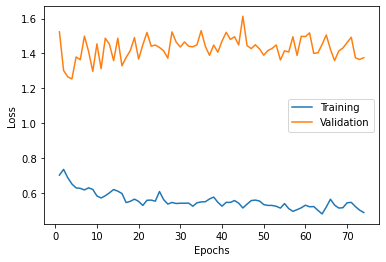
\includegraphics[width=\textwidth]{Latex template for Project Report-20220108/immagini/L2DropEarlyCWLoss.png}
         \caption{L2-Dr-ES-CW Loss}
         \label{fig:L2DropESCWLoss}
     \end{subfigure}
     \hspace{2em}
     \begin{subfigure}[b]{0.32\textwidth}
         \centering
         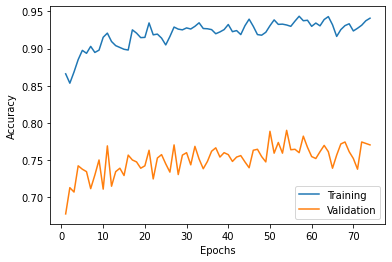
\includegraphics[width=\textwidth]{Latex template for Project Report-20220108/immagini/L2DropEarlyCWAccuracy.png}
         \caption{L2-Dr-ES-CW Acc}
         \label{fig:L2DropESCWAcc}
     \end{subfigure}
     
     \caption{Loss e accuracy dei modelli con combinazioni di regolarizzazione}
     \label{fig:secondiModelli}
\end{figure} 

Si può notare come tutti i modelli riportino risultati molto simili: ottimi valori di \textit{loss} e \textit{accuracy} sul train set, \textit{validation loss} intorno a 1.2-1.3 e \textit{validation accuracy} tra 0.75 e 0.80.

\begin{table}[h!]
\centering
\resizebox{.8\textwidth}{!}{%
        \begin{tabular}{| c | c | c | c | c |}
            \hline 
            Modello & Train Loss & Train Accuracy & Validation Loss & Validation Accuracy\\ \hline
            FAMD  & 0.006 & 0.999 & 2.594 & 0.749 \\ \hline
            OHE & 0.002 & 0.999 & 1.839 & 0.822 \\ \hline
            L1 & 0.391 & 0.961 & 1.377 & 0.793 \\ \hline
            L2 & 0.354 & 0.971 & 1.171 & 0.782 \\ \hline
            L2-Dropout & 0.498 & 0.910 & 1.208 & 0.764 \\ \hline
            L2-ES & 0.516 & 0.897 & 1.052 & 0.756 \\ \hline
            L2-Dropout-ES & 0.387 & 0.957 & 1.241 & 0.785 \\ \hline
            L2-ES-CW & 0.449 & 0.967 & 1.290 & 0.771 \\ \hline
            L2-Dropout-ES-CW & 0.405 & 0.971 & 1.363 & 0.790 \\ \hline
        \end{tabular}
        }
    \caption{Risultati all'ultima epoca su Train e Validation set}
    \label{tab:xxx}
\end{table}

Dall'osservazione dei grafici in Figura \ref{fig:primiModelli} e Figura \ref{fig:secondiModelli}, non avendo riscontrato alcun modello di spicco tra gli altri, ne sono stati selezionati tre per proseguire l'analisi dei loro risultati: \textit{L2}, \textit{L2 ES} (che riporta il più basso valore di \textit{accuracy loss} tra tutti i modelli) e \textit{L2 ES CW}.
Per questi, verranno infatti valutate alcune misure di performance su validation e test set, visibili in Tabella \ref{table:l2m}. 
È possibile notare come i valori ottenuti, per questi tre modelli, con il test set siano leggermente peggiori rispetto a quelli ottenuti con il validation set, ma molto simili. 
In particolare si osservano difficoltà nella predizione della classe 2, \textit{test accuracy} intorno a 0.74 e \textit{test loss} tra 1.20 e 1.60.

% \begin{figure}[H]
%         \centering
%      \begin{subfigure}[b]{0.27\textwidth}
%          \centering
%          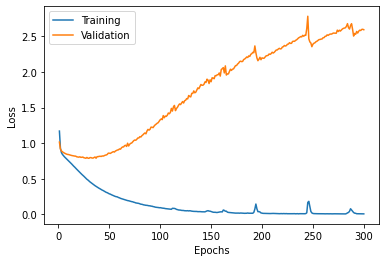
\includegraphics[width=\textwidth]{Latex template for Project Report-20220108/immagini/FAMDLoss.PNG}
%          %\captionsize{small}
%          \caption{FAMD Loss}
%          \label{fig:FAMDLoss}
%      \end{subfigure}
%      \hfill
%      \begin{subfigure}[b]{0.27\textwidth}
%          \centering
%          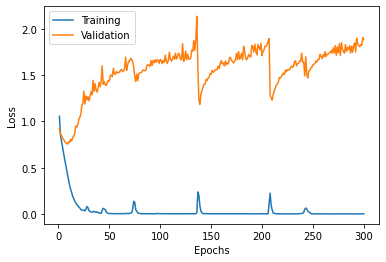
\includegraphics[width=\textwidth]{Latex template for Project Report-20220108/immagini/OHELoss.png}
%          \caption{OHE Loss}
%          \label{fig:OHELoss}
%      \end{subfigure}
%      \hfill
%      \begin{subfigure}[b]{0.27\textwidth}
%          \centering
%          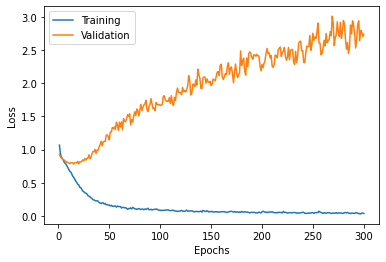
\includegraphics[width=\textwidth]{Latex template for Project Report-20220108/immagini/DropoutLoss.png}
%          \caption{Dropout Loss}
%          \label{fig:DropLoss}
%      \end{subfigure}
     
%      \begin{subfigure}[b]{0.27\textwidth}
%          \centering
%          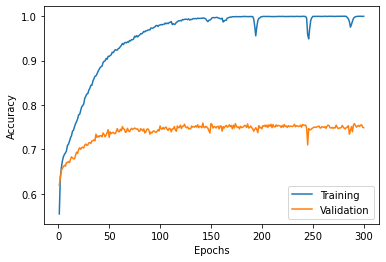
\includegraphics[width=\textwidth]{Latex template for Project Report-20220108/immagini/FAMDAccuracy.png}
%          \caption{FAMD Accuracy}
%          \label{fig:FAMDAcc}
%      \end{subfigure}
%      \hfill
%      \begin{subfigure}[b]{0.27\textwidth}
%          \centering
%          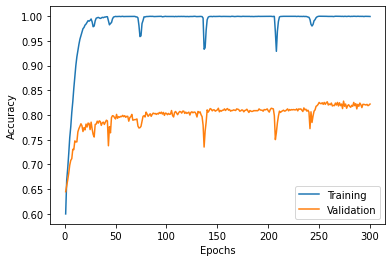
\includegraphics[width=\textwidth]{Latex template for Project Report-20220108/immagini/OHEAccuracy.png}
%          \caption{OHE Accuracy}
%          \label{fig:OHEAcc}
%      \end{subfigure}
%      \hfill
%      \begin{subfigure}[b]{0.27\textwidth}
%          \centering
%          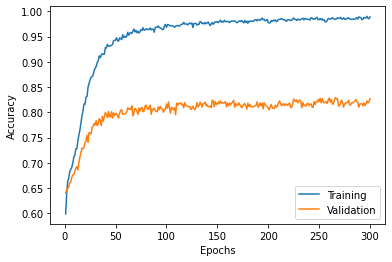
\includegraphics[width=\textwidth]{Latex template for Project Report-20220108/immagini/DropoutAccuracy.png}
%          \caption{Dropout Accuracy}
%          \label{fig:DropAcc}
%      \end{subfigure}

% \end{figure}




%Al fine di rendere ancora più chiaro il risultato ottenuto all'ultima epoca da ogni modello, sono stati riportati nella Tabella \ref{tab:xxx} i valori di \textit{loss} e \textit{accuracy} per train e validation set.


%%%%%%%%%%tabella multi row
% richiesti: 
% \usepackage{adjustbox}
% \usepackage{multirow}
% \begin{table}[h!]
% \centering
% \resizebox{.45\textwidth}{!}{%
%         \begin{tabular}{| c | c | c | c |}
%             \hline 
%             \multicolumn{1}{|c|}{Modello} & \multicolumn{1}{c|}{Set} & \multicolumn{1}{c|}{Loss} & \multicolumn{1}{c|}{Accuracy}\\ \hline
%             \multirow{2}{*}{FAMD}  &
%             \multicolumn{1}{l|}{Train} & \multicolumn{1}{l|}{0.006} & \multicolumn{1}{c|}{0.999} \\ \cline{2-4}
%                                       & \multicolumn{1}{l|}{Validation} & \multicolumn{1}{l|}{2.594} & \multicolumn{1}{c|}{0.749} \\ \hline
%             \multirow{2}{*}{OHE} & 
%             \multicolumn{1}{l|}{Train} & \multicolumn{1}{l|}{0.002} & \multicolumn{1}{c|}{0.999} \\ \cline{2-4}
%                                       & \multicolumn{1}{l|}{Validation} & \multicolumn{1}{l|}{1.839} & \multicolumn{1}{c|}{0.822} \\ \hline
%             \multirow{2}{*}{L1} &
%             \multicolumn{1}{l|}{Train} & \multicolumn{1}{l|}{0.391} & \multicolumn{1}{c|}{0.961} \\ \cline{2-4}
%                                       & \multicolumn{1}{l|}{Validation} & \multicolumn{1}{l|}{1.377} & \multicolumn{1}{c|}{0.793} \\ \hline
%             \multirow{2}{*}{L2} &
%             \multicolumn{1}{l|}{Train} & \multicolumn{1}{l|}{0.354} & \multicolumn{1}{c|}{0.971} \\ \cline{2-4}
%                                       & \multicolumn{1}{l|}{Validation} & \multicolumn{1}{l|}{1.171} & \multicolumn{1}{c|}{0.782} \\ \hline
%             \multirow{2}{*}{L2-Dropout} &
%             \multicolumn{1}{l|}{Train} & \multicolumn{1}{l|}{0.498} & \multicolumn{1}{c|}{0.910} \\ \cline{2-4}
%                                       & \multicolumn{1}{l|}{Validation} & \multicolumn{1}{l|}{1.208} & \multicolumn{1}{c|}{0.764} \\ \hline
%             \multirow{2}{*}{L2-ES} &
%             \multicolumn{1}{l|}{Train} & \multicolumn{1}{l|}{0.516} & \multicolumn{1}{c|}{0.897} \\ \cline{2-4}
%                                       & \multicolumn{1}{l|}{Validation} & \multicolumn{1}{l|}{1.052} & \multicolumn{1}{c|}{0.756} \\ \hline
%             \multirow{2}{*}{L2-Dropout-ES} &
%             \multicolumn{1}{l|}{Train} & \multicolumn{1}{l|}{0.387} & \multicolumn{1}{c|}{0.957} \\ \cline{2-4}
%                                       & \multicolumn{1}{l|}{Validation} & \multicolumn{1}{l|}{1.241} & \multicolumn{1}{c|}{0.785} \\ \hline
%             \multirow{2}{*}{L2-ES-CW} &
%             \multicolumn{1}{l|}{Train} & \multicolumn{1}{l|}{0.449} & \multicolumn{1}{c|}{0.967} \\ \cline{2-4}
%                                       & \multicolumn{1}{l|}{Validation} & \multicolumn{1}{l|}{1.290} & \multicolumn{1}{c|}{0.771} \\ \hline
%             \multirow{2}{*}{L2-Dropout-ES-CW} &
%             \multicolumn{1}{l|}{Train} & \multicolumn{1}{l|}{0.405} & \multicolumn{1}{c|}{0.971} \\ \cline{2-4}
%                                       & \multicolumn{1}{l|}{Validation} & \multicolumn{1}{l|}{1.363} & \multicolumn{1}{c|}{0.790} \\ \hline
%         \end{tabular}
%         }
%     \caption{Risultati all'ultima epoca su Train e Validation set}
%     \label{tab:xxx}
% \end{table}





%Si può notare come tutti i modelli riportino risultati molto simili: ottimi valori di \textit{loss} e \textit{accuracy} sul train set, \textit{validation loss} intorno a 1.2-1.3 e \textit{validation accuracy} tra 0.75 e 0.80.

%Dall'osservazione dei grafici in Figura \ref{fig:primiModelli} e Figura \ref{fig:secondiModelli}, non avendo riscontrato alcun modello di spicco tra gli altri, ne sono stati selezionati tre per proseguire l'analisi dei loro risultati: \textit{L2}, \textit{L2 EarlyStopping} (che riporta il più basso valore di \textit{accuracy loss} tra tutti i modelli) e \textit{L2 EarlyStopping ClassWeight}.
%Per questi, verranno infatti valutate alcune misure di performance su validation e test set, visibili in Tabella \ref{table:l2m}. 

% \begin{figure}[H]
%      \centering
%      \begin{subfigure}[b]{0.3\textwidth}
%          \centering
%          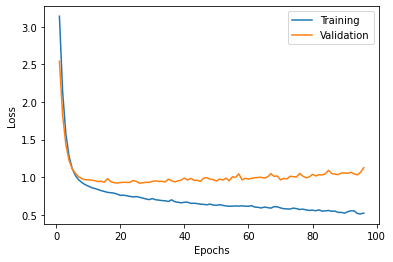
\includegraphics[width=\textwidth]{Latex template for Project Report-20220108/immagini/L2EarlyLoss.png}
%          \caption{L2-ES Loss}
%          \label{fig:L2ESLoss}
%      \end{subfigure}
%      \hspace{2em}
%      \begin{subfigure}[b]{0.3\textwidth}
%          \centering
%          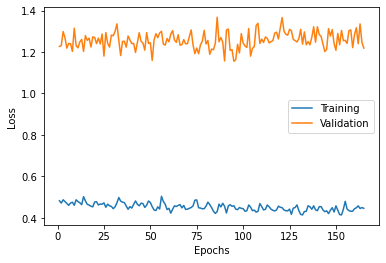
\includegraphics[width=\textwidth]{Latex template for Project Report-20220108/immagini/L2DropEarlyLoss.png}
%          \caption{L2-Dr-ES Loss}
%          \label{fig:L2DropESLoss}
%      \end{subfigure}
     
%      \begin{subfigure}[b]{0.3\textwidth}
%          \centering
%          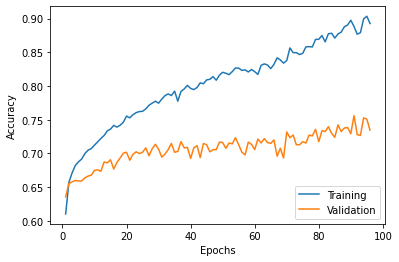
\includegraphics[width=\textwidth]{Latex template for Project Report-20220108/immagini/L2EarlyAccuracy.png}
%          \caption{L2-ES Accuracy}
%          \label{fig:L2ESAcc}
%      \end{subfigure}
%      \hspace{2em}
%      \begin{subfigure}[b]{0.3\textwidth}
%          \centering
%          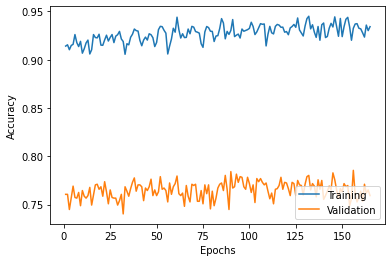
\includegraphics[width=\textwidth]{Latex template for Project Report-20220108/immagini/L2DropEarlyAccuracy.png}
%          \caption{L2-Dr-ES Accuracy}
%          \label{fig:L2DropESAcc}
%      \end{subfigure}
     
%      \begin{subfigure}[b]{0.3\textwidth}
%          \centering
%          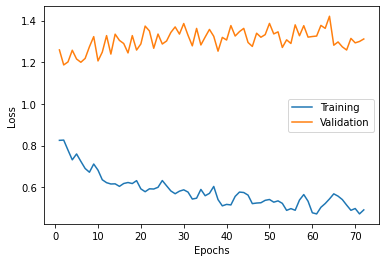
\includegraphics[width=\textwidth]{Latex template for Project Report-20220108/immagini/L2EarlyCWLoss.png}
%          \caption{L2-ES-CW Loss}
%          \label{fig:L2ESCWLoss}
%      \end{subfigure}
%      \hspace{2em}
%      \begin{subfigure}[b]{0.3\textwidth}
%          \centering
%          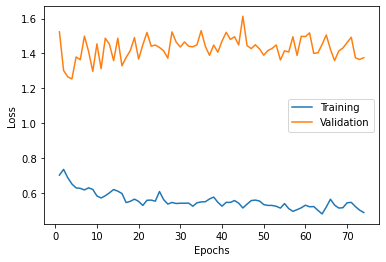
\includegraphics[width=\textwidth]{Latex template for Project Report-20220108/immagini/L2DropEarlyCWLoss.png}
%          \caption{L2-Dr-ES-CW Loss}
%          \label{fig:L2DropESCWLoss}
%      \end{subfigure}
     
%      \begin{subfigure}[b]{0.3\textwidth}
%          \centering
%          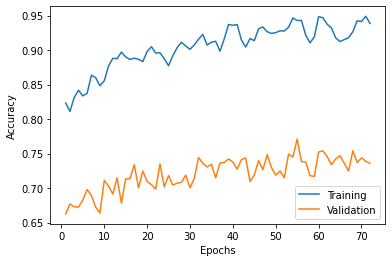
\includegraphics[width=\textwidth]{Latex template for Project Report-20220108/immagini/L2EarlyCWAccuracy.png}
%          \caption{L2-ES-CW Acc}
%          \label{fig:L2ESCWAcc}
%      \end{subfigure}
%      \hspace{2em}
%      \begin{subfigure}[b]{0.3\textwidth}
%          \centering
%          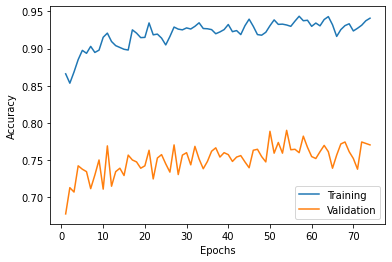
\includegraphics[width=\textwidth]{Latex template for Project Report-20220108/immagini/L2DropEarlyCWAccuracy.png}
%          \caption{L2-Dr-ES-CW Acc}
%          \label{fig:L2DropESCWAcc}
%      \end{subfigure}
     
%      \caption{Loss e accuracy dei modelli ottenuti combinando diverse tecniche di regolarizzazione}
%         %\label{fig:three graphs}
% \end{figure}






% \begin{table}[H]
% \centering
%         \begin{tabular}{| c | c | c | c |}
%             \hline 
%             \multicolumn{1}{|c|}{Modello} & \multicolumn{1}{c|}{Set} & \multicolumn{1}{c|}{Loss} & \multicolumn{1}{c|}{Accuracy}\\ \hline
%             \multirow{2}{*}{FAMD}  &
%             \multicolumn{1}{l|}{Train} & \multicolumn{1}{l|}{0.006} & \multicolumn{1}{l|}{0.999} \\ \cline{2-4}
%                                       & \multicolumn{1}{l|}{Validation} & \multicolumn{1}{l|}{2.594} & \multicolumn{1}{l|}{0.749} \\ \hline
%             \multirow{2}{*}{OHE} & 
%             \multicolumn{1}{l|}{Train} & \multicolumn{1}{l|}{0.002} & \multicolumn{1}{l|}{0.999} \\ \cline{2-4}
%                                       & \multicolumn{1}{l|}{Validation} & \multicolumn{1}{l|}{1.839} & \multicolumn{1}{l|}{0.822} \\ \hline
%             \multirow{2}{*}{L1} &
%             \multicolumn{1}{l|}{Train} & \multicolumn{1}{l|}{0.391} & \multicolumn{1}{l|}{0.961} \\ \cline{2-4}
%                                       & \multicolumn{1}{l|}{Validation} & \multicolumn{1}{l|}{1.377} & \multicolumn{1}{l|}{0.793} \\ \hline
%             \multirow{2}{*}{L2} &
%             \multicolumn{1}{l|}{Train} & \multicolumn{1}{l|}{0.354} & \multicolumn{1}{l|}{0.971} \\ \cline{2-4}
%                                       & \multicolumn{1}{l|}{Validation} & \multicolumn{1}{l|}{1.171} & \multicolumn{1}{l|}{0.782} \\ \hline
%             \multirow{2}{*}{L2-Dropout} &
%             \multicolumn{1}{l|}{Train} & \multicolumn{1}{l|}{0.498} & \multicolumn{1}{l|}{0.910} \\ \cline{2-4}
%                                       & \multicolumn{1}{l|}{Validation} & \multicolumn{1}{l|}{1.208} & \multicolumn{1}{l|}{0.764} \\ \hline
%             \multirow{2}{*}{L2-Early Stopping} &
%             \multicolumn{1}{l|}{Train} & \multicolumn{1}{l|}{0.516} & \multicolumn{1}{l|}{0.897} \\ \cline{2-4}
%                                       & \multicolumn{1}{l|}{Validation} & \multicolumn{1}{l|}{1.052} & \multicolumn{1}{l|}{0.756} \\ \hline
%             \multirow{2}{*}{L2-Dropout-Early Stopping} &
%             \multicolumn{1}{l|}{Train} & \multicolumn{1}{l|}{0.387} & \multicolumn{1}{l|}{0.957} \\ \cline{2-4}
%                                       & \multicolumn{1}{l|}{Validation} & \multicolumn{1}{l|}{1.241} & \multicolumn{1}{l|}{0.785} \\ \hline
%             \multirow{2}{*}{L2-Early Stopping-Class Weight} &
%             \multicolumn{1}{l|}{Train} & \multicolumn{1}{l|}{0.449} & \multicolumn{1}{l|}{0.967} \\ \cline{2-4}
%                                       & \multicolumn{1}{l|}{Validation} & \multicolumn{1}{l|}{1.290} & \multicolumn{1}{l|}{0.771} \\ \hline
%             \multirow{2}{*}{L2-Dropout-Early Stopping-Class Weight} &
%             \multicolumn{1}{l|}{Train} & \multicolumn{1}{l|}{0.405} & \multicolumn{1}{l|}{0.971} \\ \cline{2-4}
%                                       & \multicolumn{1}{l|}{Validation} & \multicolumn{1}{l|}{1.363} & \multicolumn{1}{l|}{0.790} \\ \hline
%         \end{tabular}
%     \caption{Risultati su Train e Validation set}
%     \label{tab:xxx}
% \end{table}



\begin{table}[h!]
    \parbox{.45\textwidth}{
        \centering
        \begin{adjustbox}{max width=.45\textwidth}
        \begin{tabular}{|c|c|c|c|c|}
        \hline
            \multicolumn{5}{| c |}{L2 Validation Set} \\ \hline
            &  precision &   recall & f1-score  &  support \\ \hline
            0   &     0.56   &    0.74  &    0.64    &    93 \\ \hline
            1   &     0.58   &    0.60  &    0.59    &    253\\ \hline
            2   &     0.56   &    0.36  &    0.44    &    306\\ \hline
            3   &     0.84   &    0.91  &    0.87    &    877\\ \hline
            accuracy   &       &        &    0.74   &   1529 \\ \hline
            loss   &     &     & 1.31   &   1529\\ \hline
            macro avg   &    0.63     & 0.65   &   0.63   &   1529 \\ \hline
            weighted avg   &    0.72    &  0.74     & 0.72   &   1529\\ \hline
        \end{tabular}
        \end{adjustbox}
    }
    \hfill
    \parbox{.45\textwidth}{
    \begin{adjustbox}{max width=.45\textwidth}
    \centering
        \begin{tabular}{|c|c|c|c|c|}
                \hline
                \multicolumn{5}{| c |}{L2 Test Set} \\ \hline
                 & precision &   recall & f1-score  &  support \\ \hline
                    0    &    0.64    &   0.75     &  0.69    &    140 \\ \hline
                   1    &   0.60    &  0.58    &  0.59    &   318\\ \hline
                   2    &   0.56    &  0.38   &   0.45    &   376\\ \hline
                   3    &   0.82    &  0.90   &   0.85   &  1078\\ \hline
            accuracy    &       &        &    0.73    &  1912\\ \hline
            loss   &     &     & 1.59   &   1912\\ \hline
           macro avg    &   0.65    &  0.65  &    0.65    &  1912\\ \hline
        weighted avg    &   0.72   &   0.73  &    0.72   &   1912\\ \hline
            \end{tabular}
            \end{adjustbox}
    }

    \vspace{.2cm}
    \parbox{.45\textwidth}{
        \centering
        \begin{adjustbox}{max width=.45\textwidth}
        \begin{tabular}{|c|c|c|c|c|}
        \hline
            \multicolumn{5}{| c |}{L2-Early Stopping Validation Set} \\ \hline
            &  precision &   recall & f1-score  &  support \\ \hline
            0   &    0.32    &  0.68    &  0.43    &    57\\ \hline
            1   &    0.57    &  0.57    &  0.57    &   263\\ \hline
            2   &    0.45   &   0.41    &  0.43     &  212\\ \hline
            3    &   0.93   &   0.88    &  0.91    &  997\\ \hline
            accuracy    &    &        &           0.76    &  1529\\ \hline
            loss   &     &     & 1.05   &   1529\\ \hline
            macro avg    &   0.57    &  0.64   &   0.58    &  1529\\ \hline
            weighted avg    &   0.78  &    0.76   &   0.76   &   1529 \\ \hline
        \end{tabular}
        \end{adjustbox}
    }
    \hfill
    \parbox{.45\textwidth}{
    \begin{adjustbox}{max width=.45\textwidth}
    \centering
        \begin{tabular}{|c|c|c|c|c|}
                \hline
                \multicolumn{5}{| c |}{L2-Early Stopping Test Set} \\ \hline
                 & precision &   recall & f1-score  &  support \\ \hline
                0  &     0.34   &   0.63    &  0.44   &     87\\ \hline
                1    &   0.53   &   0.49    &  0.51 &      335\\ \hline
                2    &   0.46   &   0.41    &  0.43 &      285\\ \hline
                3    &   0.89   &   0.88    &  0.89 &     1205\\ \hline
                accuracy   &    &   &  0.73   &   1912\\ \hline
                loss   &     &     & 1.20   &   1912\\ \hline
                macro avg   &    0.55   &   0.60  &    0.57   &   1912\\ \hline
                weighted avg   &    0.74    &  0.73    &  0.73   &   1912\\ \hline
            \end{tabular}
            \end{adjustbox}
    }
    
    \vspace{.2cm}
    \parbox{.45\textwidth}{
        \centering
        \begin{adjustbox}{max width=.45\textwidth}
        \begin{tabular}{|c|c|c|c|c|}
        \hline
            \multicolumn{5}{| c |}{L2-Early Stopping-Class Weight Validation Set} \\ \hline
            &  precision &   recall & f1-score  &  support \\ \hline
            0   &    0.50  &    0.82  &    0.62   &     76\\ \hline
            1   &    0.66  &    0.63  &    0.64   &    276\\ \hline
            2   &    0.62  &    0.43  &    0.51   &    284\\ \hline
            3   &    0.87  &    0.92  &    0.89   &    893\\ \hline
            accuracy   &    &         &    0.77   &   1529\\ \hline
            loss   &     &     & 1.29   &   1529\\ \hline
            macro avg  & 0.66  &  0.70 & 0.67   &   1529\\ \hline
            weighted avg   &     0.77    &   0.77    &   0.76    &   1529\\ \hline
        \end{tabular}
        \end{adjustbox}
    }
    \hfill
    \parbox{.45\textwidth}{
    \begin{adjustbox}{max width=.45\textwidth}
    \centering
        \begin{tabular}{|c|c|c|c|c|}
                \hline
                \multicolumn{5}{| c |}{L2-Early Stopping-Class Weight Test Set} \\ \hline
                 & precision &   recall & f1-score  &  support \\ \hline
                0   &    0.55  &    0.73  &    0.63   &    124\\ \hline
                1   &    0.59  &    0.56  &    0.58   &    329\\ \hline
                2   &    0.60  &    0.42  &    0.50   &    359\\ \hline
                3   &    0.84  &    0.91  &    0.87   &   1100\\ \hline
                accuracy   &    &         & 0.75   &   1912\\ \hline
                loss   &     &     & 1.56   &   1912\\ \hline
                macro avg    &   0.65   &   0.66   &   0.65   &   1912\\ \hline
                weighted avg    &   0.74    &  0.75    &  0.74   &   1912\\ \hline
            \end{tabular}
            \end{adjustbox}
    }
        \caption{Risultati Validation e Test set}
        \label{table:l2m}
\end{table}

%È possibile notare come i valori ottenuti, per questi tre modelli, con il test set siano leggermente peggiori rispetto a quelli ottenuti con il validation set, ma molto simili. 
%In particolare si osservano difficoltà nella predizione della classe 2, \textit{test accuracy} intorno a 0.74 e \textit{test loss} tra 1.20 e 1.60.
\section{Discussione}
%\textit{The discussion section aims at interpreting the results in light of the project's objectives. The most important goal of this section is to interpret the results so that the reader is informed of the insight or answers that the results provide. This section should also present an evaluation of the particular approach taken by the group. For example: Based on the results, how could the experimental procedure be improved? What additional, future work may be warranted? What recommendations can be drawn?}

Dai risultati riportati nella Tabella \ref{table:l2m} è possibile effettuare un'analisi più approfondita dei 3 modelli selezionati: \textit{L2}, \textit{L2 ES} e \textit{L2 ES CW}.
I risultati del modello \textit{L2} ottenuti sul validation set indicano che la rete riconosce molto bene la classe 3, data la maggior quantità di dati utilizzati nell'addestramento (maggior supporto), mentre fatica a riconoscere le restanti classi. 
In particolare viene mal predetta la classe 2 per cui si ha una recall particolarmente bassa (pari a 0.36). 
In generale però, ad eccezione della classe 2, la precision tende ad avere valori più bassi della recall. 
Nelle misure di performance sul test set è possibile notare risultati molto simili se non leggermente migliori rispetto a quelli ottenuti sul validation set.
La \textit{test accuracy} risulta pressoché identica mentre la \textit{test loss} risulta leggermente peggiorata. 
In generale entrambe le misure risultano essere buone ma non ottimali.
I risultati del modello \textit{L2 ES} risultano essere i migliori ottenuti.
\textit{validation loss} e \textit{validation accuracy} riportano valori migliori rispetto a quelli ottenuti con il modello L2, anche se non ancora ottimali (accuratezza del 76\%). 
In questo caso la classe predetta in maniera peggiore risulta essere la classe 0 (precision pari a 0.32), ma si ottengono nuovamente scarsi risultati anche sulla classe 2. L'unica classe predetta ottimamente è la 3, sempre grazie al grande supporto.
Sul test set i risultati ottenuti sono molto simili ma leggermente peggiori. In definitiva si può comunque affermare che questo sia il modello migliore con una \textit{test accuracy} del 73\% e un \textit{test loss} di 1.20. 
I risultati del modello \textit{L2 ES CW} per validation e test set sono simili ai precedenti modelli. Benché la classe 3 sia sempre quella predetta meglio e la 2 quella con i peggior risultati, si riscontra in questo caso un generale miglioramento nella predizione delle singole classi (valori maggiori di f1-score). Ciò è dovuto all'azione di \textit{CW}, che pur non incidendo moltissimo, contribuisce almeno in parte a questo miglioramento.
Inoltre, con questo modello otteniamo i valori più alti per l'\textit{accuracy} sia di validation che di test set (rispettivamente 77\% e 75\%).
I valori di \textit{loss} sia per validation che per test set risultano invece molto simili a quelli del modello \textit{L2} e quindi peggiori di quelli di \textit{L2 ES}.
\section{Conclusioni}
%\textit{Conclusions should summarize the central points made in the Discussion section, reinforcing for the reader the value and implications of the work. If the results were not definitive, specific future work that may be needed can be (briefly) described. The conclusions should never contain ``surprises''. Therefore, any conclusions should be based on observations and data already discussed. It is considered extremely bad form to introduce new data in the conclusions.}

In conclusione nessuno dei modelli precedentemente sperimentati risalta tra gli altri per le proprie performance. Si potrebbe evidenziare il modello \textit{L2 ES} come quello che ottiene una \textit{loss} migliore o il modello \textit{L2 ES CW} come quello che ottiene una buona \textit{accuracy}, ma i risultati ottenuti non differiscono in modo significativo gli uni dagli altri.
L'\textit{accuracy} in fase di validation si attesta circa sul 76\%, mentre sul test set sul 74\%. La \textit{loss} rimane sopra 1 in tutti i modelli testati.
Nonostante le numerose tecniche testate, le reti testate producono risultati buoni ma non soddisfacenti e necessitano pertanto di ulteriori migliorie o a livello di dati o a livello di struttura della rete. 

%\section*{References}

%\textit{The references section should contain complete citations following standard form.  The references should be numbered and listed in the order they were cited in the body of the report. In the text of the report, a particular reference can be cited by using a numerical number in brackets as \cite{Lee2015} that corresponds to its number in the reference list. \LaTeX provides several styles to format the references}


\bibliographystyle{IEEEtran}
\bibliography{references.bib}

\end{document}